% ---
% school: "college"
% level: "8eme"
% section: null
% chapter: "التناظر المركزي"
% source: "Axiomaths"
% title: "مراكز التناظر ومحاوره"
% country: "Tunisie"
% year: 2026
% professor: "Axiomaths"
% difficulty: "Moyen"
% points: null
% tags: ["centre-de-symetrie", "axe-de-symetrie", "hexagone", "quadrilateres"]
% ---
% Exercice 10/19 de la série 8ème « التناظر المركزي » (statement + \axsol + solution). Compiler avec XeLaTeX + axiomath.sty (+ axiomaths-logo.png).
\documentclass[12pt,a4paper]{article}
\usepackage[level=8b,color=15803D]{axiomath}
\usetikzlibrary{arrows.meta}
\newcommand{\cm}{\,\mathrm{cm}}
\axsetup{title={التناظر المركزي}, corrige}

\begin{document}

\begin{corr}[title={مراكز التناظر ومحاوره}, stars=3, source={Axiomaths}]
\begin{enumerate}
  \item أتمم الجدول :
  \begin{center}
  \renewcommand{\arraystretch}{1.5}
  \begin{tabular}{|c|c|c|}
    \hline
    الشكل & يقبل مركز تناظر ؟ & عدد محاور التناظر \\ \hline
    متوازي أضلاع (غير مستطيل وغير معين) & \phantom{لا نهاية} & \phantom{لا نهاية} \\ \hline
    مستطيل (غير مربع) & & \\ \hline
    معين (غير مربع) & & \\ \hline
    مثلث متقايس الضلعين (غير متقايس الأضلاع) & & \\ \hline
    شبه منحرف عادي & & \\ \hline
    دائرة & & \\ \hline
  \end{tabular}
  \end{center}
  \item السداسي $ABCDEF$ مرسوم على الشبكة. بين أن له مركز تناظر $O$ يُطلب تعيينه.
  \begin{center}
  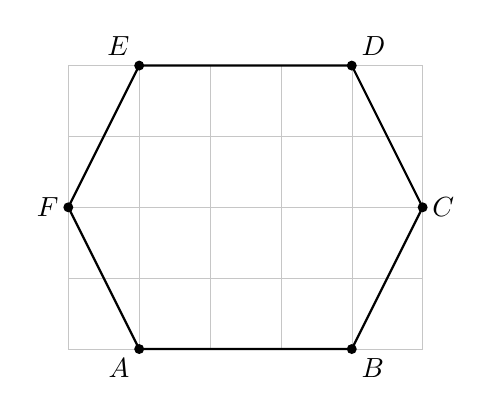
\begin{tikzpicture}[scale=0.9]
    \draw[gray!45,very thin] (0,0) grid (5,4);
    \draw[thick] (1,0)--(4,0)--(5,2)--(4,4)--(1,4)--(0,2)--cycle;
    \fill (1,0) circle (2pt) node[below left] {$A$};
    \fill (4,0) circle (2pt) node[below right] {$B$};
    \fill (5,2) circle (2pt) node[right] {$C$};
    \fill (4,4) circle (2pt) node[above right] {$D$};
    \fill (1,4) circle (2pt) node[above left] {$E$};
    \fill (0,2) circle (2pt) node[left] {$F$};
  \end{tikzpicture}
  \end{center}
  \item عيّن محوري تناظر للسداسي $ABCDEF$.
  \item هل كل شكل يقبل مركز تناظر يقبل محور تناظر ؟ وهل العكس صحيح ؟
\end{enumerate}
\axsol
\begin{enumerate}[itemsep=14pt]
  \item\leavevmode
  \begin{prop}[مركز تناظر شكل]
  $O$ مركز تناظر شكل $\mathcal{F}$ معناه \ib{مناظر $\mathcal{F}$ بالنسبة إلى $O$ هو $\mathcal{F}$ نفسه}.
  \end{prop}
  \begin{center}
  \renewcommand{\arraystretch}{1.5}
  \begin{tabular}{|c|c|c|}
    \hline
    الشكل & يقبل مركز تناظر ؟ & عدد محاور التناظر \\ \hline
    متوازي أضلاع (غير مستطيل وغير معين) & نعم & 0 \\ \hline
    مستطيل (غير مربع) & نعم & 2 \\ \hline
    معين (غير مربع) & نعم & 2 \\ \hline
    مثلث متقايس الضلعين (غير متقايس الأضلاع) & لا & 1 \\ \hline
    شبه منحرف عادي & لا & 0 \\ \hline
    دائرة & نعم & لا نهاية \\ \hline
  \end{tabular}
  \end{center}
  لمتوازي الأضلاع (والمستطيل والمعين) مركز هو نقطة تقاطع قطريه ؛ وللدائرة مركز هو مركزها.
  \item نبحث عن نقطة تكون منتصف القطع الواصلة بين الرؤوس المتقابلة. على الشبكة : من $A$ إلى $D$ ننتقل 3 وحدات يمينا و 4 إلى الأعلى ؛ من $B$ إلى $E$ : 3 وحدات يسارا و 4 إلى الأعلى ؛ من $C$ إلى $F$ : 5 وحدات يسارا. في الحالات الثلاث تقع النقطة $O$ (المبينة على الشكل) في منتصف الانتقال، أي $O$ منتصف كل من $[AD]$ و $[BE]$ و $[CF]$.
  إذن $S_O(A)=D$ و $S_O(B)=E$ و $S_O(C)=F$ ، فمناظر السداسي هو $DEFABC$ أي السداسي نفسه. \ib{$O$ مركز تناظر السداسي}.
  \begin{center}
  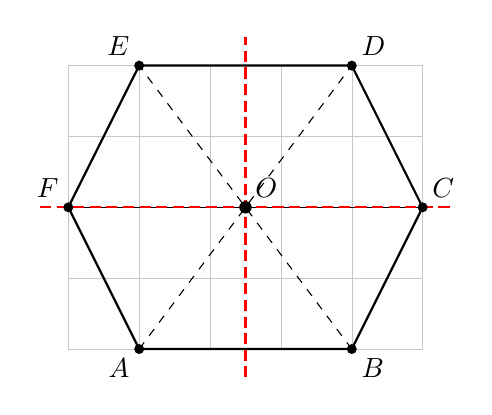
\begin{tikzpicture}[scale=0.9]
    \draw[gray!45,very thin] (0,0) grid (5,4);
    \draw[thick] (1,0)--(4,0)--(5,2)--(4,4)--(1,4)--(0,2)--cycle;
    \draw[dashed] (1,0)--(4,4);
    \draw[dashed] (4,0)--(1,4);
    \draw[dashed] (5,2)--(0,2);
    \draw[red,thick,dash pattern=on 4pt off 2pt] (2.5,-0.4)--(2.5,4.4);
    \draw[red,thick,dash pattern=on 4pt off 2pt] (-0.4,2)--(5.4,2);
    \fill (1,0) circle (2pt) node[below left] {$A$};
    \fill (4,0) circle (2pt) node[below right] {$B$};
    \fill (5,2) circle (2pt) node[above right] {$C$};
    \fill (4,4) circle (2pt) node[above right] {$D$};
    \fill (1,4) circle (2pt) node[above left] {$E$};
    \fill (0,2) circle (2pt) node[above left] {$F$};
    \fill (2.5,2) circle (2.5pt) node[above right] {$O$};
  \end{tikzpicture}
  \end{center}
  \item المستقيم العمودي المنصّف لـ $[AB]$ (الذي يمر من $O$) يحوّل $A$ إلى $B$ و $F$ إلى $C$ و $E$ إلى $D$ : إنه محور تناظر. والمستقيم الأفقي المار من $O$ يحوّل $A$ إلى $E$ و $B$ إلى $D$ و $F$ و $C$ كل منهما إلى نفسه : إنه محور ثانٍ. \ib{المحوران متعامدان ويتقاطعان في $O$}.
  \item لا في الاتجاهين :
  \begin{itemize}
    \item متوازي الأضلاع العادي له مركز تناظر ولا محور له.
    \item المثلث المتقايس الضلعين له محور تناظر ولا مركز له.
  \end{itemize}
  \textbf{الفكرة :} لا تلازم بين المركز والمحور ؛ وإذا كان لشكل محوران متعامدان فنقطة تقاطعهما مركز تناظره (كما في السداسي والمعين والمستطيل).
\end{enumerate}
\end{corr}

\end{document}
